\documentclass[../5RO17_TP4.tex]{subfiles}

\begin{document}
\section{Décimation de nuages de points}
\noindent Lorsqu'on traite des nuages de points volumineux et denses, le sous-échantillonnage par décimation peut être une solution efficace pour réduire la quantité de données tout en conservant une représentation représentative. La décimation sélectionne un point tous les \texttt{k} dans le nuage, ce qui permet de conserver l'essentiel de la structure tout en réduisant la complexité des calculs nécessaires pour les manipulations.\\

\noindent Chaque point du nuage est représenté par une ligne contenant les coordonnées $x$, $y$ et $z$. Traditionnellement, on pourrait réaliser cette décimation en parcourant les points de manière itérative et en ajoutant au nouvel ensemble de données chaque \texttt{i}-ème point.\\

\noindent Cependant, une approche plus concise consiste à utiliser la notation de sous-tableaux fournie par \texttt{numpy}, qui permet de sélectionner directement chaque \texttt{i}-ème ligne du tableau de coordonnées. Cette approche assure une manipulation plus rapide et efficace, particulièrement pour les grands nuages de points, en réduisant la surcharge computationnelle. Les deux méthodes d'implémentation, itérative et vectorielle, sont illustrées ci-dessous:\\

\begin{scriptsize}\mycode
	\begin{lstlisting}[language=Python, caption=\texttt{decimate()}]
def decimate(points: np.ndarray[float], k: int = 10, method: str = 'for') -> np.ndarray[float]:
    decimated_for = []

    match method.upper():
        case 'FOR':
            for i in range(0, points.shape[1], k):
                decimated_for.append(points[:, i])
        case 'NP':
            return points[:, ::k]

    return np.column_stack(decimated_for)
	\end{lstlisting}
\end{scriptsize}

\noindent En utilisant les fonctions de visualisation implémentées précédemment, il est possible d’afficher ces sous-échantillons moins denses pour une comparaison directe avec l'ensemble de données initial.
\begin{figure}[H]
    \centering
    \begin{subfigure}[b]{0.475\textwidth}
        \centering
        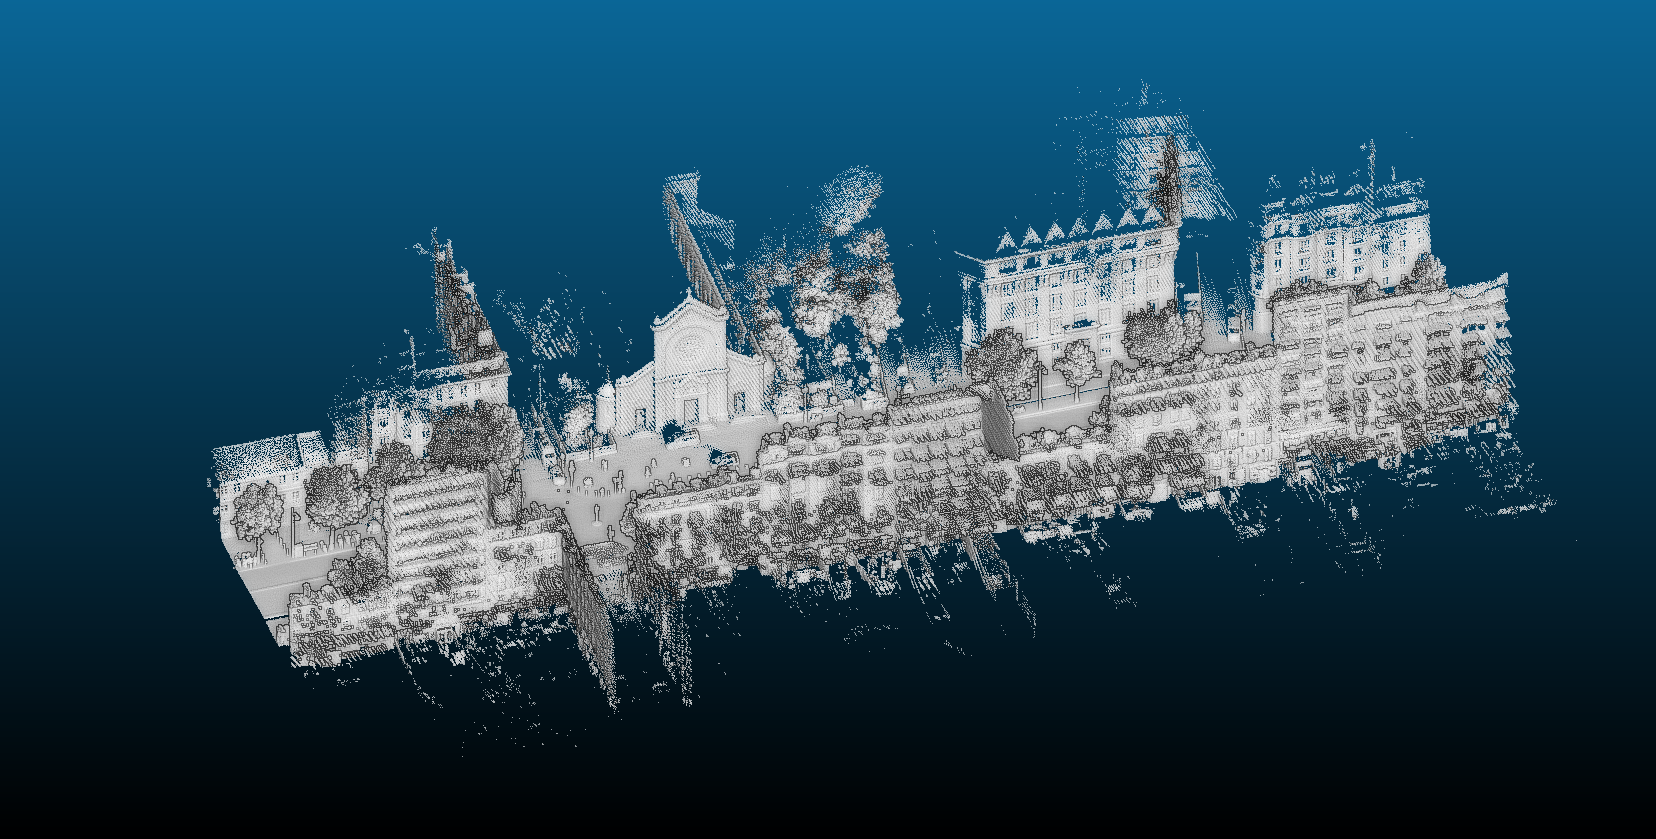
\includegraphics[width=\linewidth]{images/ndc_7.png}
        \caption{sans décimation, perspective}
        \label{}
    \end{subfigure}\hfill
    \begin{subfigure}[b]{0.475\textwidth}
        \centering
        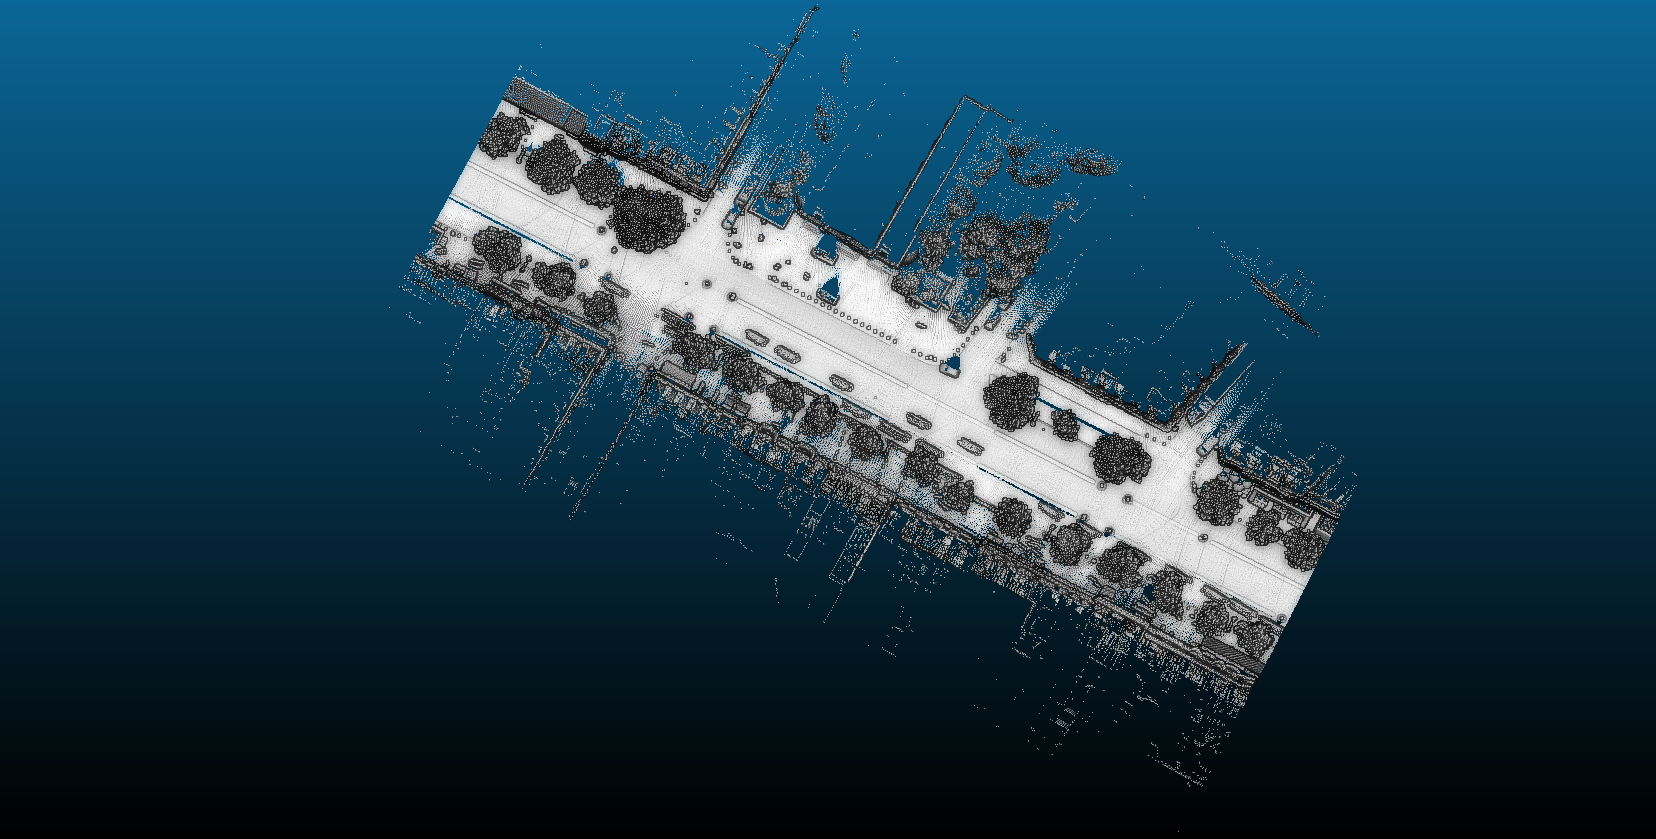
\includegraphics[width=\linewidth]{images/ndc_8.png}
        \caption{sans décimation, plan xy}
        \label{}
    \end{subfigure}\hfill
        \begin{subfigure}[b]{0.475\textwidth}
        \centering
        
\includegraphics[width=\linewidth]{images/ndc_1000_7.png}
        \caption{avec décimation $k = 1000$, perspective}
        \label{}
    \end{subfigure}\hfill
    \begin{subfigure}[b]{0.475\textwidth}
        \centering
        
\includegraphics[width=\linewidth]{images/ndc_1000_8.png}
        \caption{avec décimation $k = 1000$, plan xy}
        \label{}
    \end{subfigure}
    \caption{Visualization sur CloudCompare de \texttt{Notre-Dame-des-Champs}}
    \label{fig:decimation_ndc}
\end{figure}
\noindent Dans la Figure \ref{fig:decimation_ndc}, on observe le scan de Notre-Dame-des-Champs, une fois avec la densité de points d'origine et une seconde fois après une décimation à un facteur de 1000, soit un échantillonnage de seulement un point tous les mille. Cette réduction permet de visualiser les structures principales tout en simplifiant considérablement le modèle, offrant une vue d’ensemble plus légère tout en préservant l’essentiel des formes architecturales.

\begin{remark}
    Aucun changement majeur n'est perceptible entre les méthodes de décimation. Les deux approches réduisent efficacement le nombre de points tout en conservant l'essentiel de la structure du nuage.\\
    
    \noindent Cela montre que les deux techniques aboutissent à des résultats visuellement comparables, même pour des réductions significatives, comme l'exemple avec un facteur de décimation de 1000.
\end{remark}
\end{document}
